\documentclass{article}


% if you need to pass options to natbib, use, e.g.:
     \PassOptionsToPackage{numbers, compress}{natbib}
% before loading neurips_2023


% % %ready for submission
%  \usepackage{style/neurips_2023}


% to compile a preprint version, e.g., for submission to arXiv, add add the
% [preprint] option:
%    \usepackage[preprint]{style/neurips_2023}


% to compile a camera-ready version, add the [final] option, e.g.:
     \usepackage{style/neurips_2023}


% to avoid loading the natbib package, add option nonatbib:
%     \usepackage[nonatbib]{style/neurips_2023}


\usepackage[utf8]{inputenc} % allow utf-8 input
\usepackage[T1]{fontenc}    % use 8-bit T1 fonts
\usepackage{hyperref}       % hyperlinks
\usepackage{url}            % simple URL typesetting
\usepackage{booktabs}       % professional-quality tables
\usepackage{amsfonts}       % blackboard math symbols
\usepackage{nicefrac}       % compact symbols for 1/2, etc.
\usepackage{microtype}      % microtypography
% \usepackage{xcolor}         % colors
\usepackage{adjustbox}
\usepackage{wrapfig}
\usepackage{enumitem}
\usepackage[normalem]{ulem}
\usepackage{comment}
%%%%%%%%%%%%%%%% ADDED BY THE AUTHORS
\usepackage[dvipsnames]{xcolor}
%%%%% NEW MATH DEFINITIONS %%%%%

\usepackage{amsmath,amsfonts,amssymb}
\usepackage{bbm}
%\theoremstyle{plain}

% \newtheorem{thm}{Theorem}
% \theoremstyle{definition}
% \newtheorem{definition}{Definition} % definition numbers are dependent on theorem numbers
% \newtheorem{ex}{Example}
% \newtheorem{cor}{Corollary}

% \newtheorem{innercustomthm}{Theorem}
% \newenvironment{customthm}[1]
%   {\renewcommand\theinnercustomthm{#1}\innercustomthm}
%   {\endinnercustomthm}

\usepackage{bm}
% \usepackage{soul} % for the hl colors

% % Mark sections of captions for referring to divisions of figures
% \newcommand{\figleft}{{\em (Left)}}
% \newcommand{\figcenter}{{\em (Center)}}
% \newcommand{\figright}{{\em (Right)}}
% \newcommand{\figtop}{{\em (Top)}}
% \newcommand{\figbottom}{{\em (Bottom)}}
% \newcommand{\captiona}{{\em (a)}}
% \newcommand{\captionb}{{\em (b)}}
% \newcommand{\captionc}{{\em (c)}}
% \newcommand{\captiond}{{\em (d)}}

% % Highlight a newly defined term
% \newcommand{\newterm}[1]{{\bf #1}}


% % Figure reference, lower-case.
% \def\figref#1{figure~\ref{#1}}
% % Figure reference, capital. For start of sentence
% \def\Figref#1{Figure~\ref{#1}}
% \def\twofigref#1#2{figures \ref{#1} and \ref{#2}}
% \def\quadfigref#1#2#3#4{figures \ref{#1}, \ref{#2}, \ref{#3} and \ref{#4}}
% % Section reference, lower-case.
% \def\secref#1{section~\ref{#1}}
% % Section reference, capital.
% \def\Secref#1{Section~\ref{#1}}
% % Reference to two sections.
% \def\twosecrefs#1#2{sections \ref{#1} and \ref{#2}}
% % Reference to three sections.
% \def\secrefs#1#2#3{sections \ref{#1}, \ref{#2} and \ref{#3}}
% % Reference to an equation, lower-case.
% \def\eqref#1{equation~\ref{#1}}
% % Reference to an equation, upper case
% \def\Eqref#1{Equation~\ref{#1}}
% % A raw reference to an equation---avoid using if possible
% \def\plaineqref#1{\ref{#1}}
% % Reference to a chapter, lower-case.
% \def\chapref#1{chapter~\ref{#1}}
% % Reference to an equation, upper case.
% \def\Chapref#1{Chapter~\ref{#1}}
% % Reference to a range of chapters
% \def\rangechapref#1#2{chapters\ref{#1}--\ref{#2}}
% % Reference to an algorithm, lower-case.
% \def\algref#1{algorithm~\ref{#1}}
% % Reference to an algorithm, upper case.
% \def\Algref#1{Algorithm~\ref{#1}}
% \def\twoalgref#1#2{algorithms \ref{#1} and \ref{#2}}
% \def\Twoalgref#1#2{Algorithms \ref{#1} and \ref{#2}}
% % Reference to a part, lower case
% \def\partref#1{part~\ref{#1}}
% % Reference to a part, upper case
% \def\Partref#1{Part~\ref{#1}}
% \def\twopartref#1#2{parts \ref{#1} and \ref{#2}}

% \def\ceil#1{\lceil #1 \rceil}
% \def\floor#1{\lfloor #1 \rfloor}
% \def\1{\bm{1}}
% \newcommand{\train}{\mathcal{D}}
% \newcommand{\valid}{\mathcal{D_{\mathrm{valid}}}}
% \newcommand{\test}{\mathcal{D_{\mathrm{test}}}}

% \def\eps{{\epsilon}}


% Random variables
\def\reta{{\textnormal{$\eta$}}}
\def\ra{{\textnormal{a}}}
\def\rb{{\textnormal{b}}}
\def\rc{{\textnormal{c}}}
\def\rd{{\textnormal{d}}}
\def\re{{\textnormal{e}}}
\def\rf{{\textnormal{f}}}
\def\rg{{\textnormal{g}}}
\def\rh{{\textnormal{h}}}
\def\ri{{\textnormal{i}}}
\def\rj{{\textnormal{j}}}
\def\rk{{\textnormal{k}}}
\def\rl{{\textnormal{l}}}
% rm is already a command, just don't name any random variables m
\def\rn{{\textnormal{n}}}
\def\ro{{\textnormal{o}}}
\def\rp{{\textnormal{p}}}
\def\rq{{\textnormal{q}}}
\def\rr{{\textnormal{r}}}
\def\rs{{\textnormal{s}}}
\def\rt{{\textnormal{t}}}
\def\ru{{\textnormal{u}}}
\def\rv{{\textnormal{v}}}
\def\rw{{\textnormal{w}}}
\def\rx{{\textnormal{x}}}
\def\ry{{\textnormal{y}}}
\def\rz{{\textnormal{z}}}

% Random vectors
\def\rvepsilon{{\mathbf{\epsilon}}}
\def\rvtheta{{\mathbf{\theta}}}
\def\rva{{\mathbf{a}}}
\def\rvb{{\mathbf{b}}}
\def\rvc{{\mathbf{c}}}
\def\rvd{{\mathbf{d}}}
\def\rve{{\mathbf{e}}}
\def\rvf{{\mathbf{f}}}
\def\rvg{{\mathbf{g}}}
\def\rvh{{\mathbf{h}}}
\def\rvu{{\mathbf{i}}}
\def\rvj{{\mathbf{j}}}
\def\rvk{{\mathbf{k}}}
\def\rvl{{\mathbf{l}}}
\def\rvm{{\mathbf{m}}}
\def\rvn{{\mathbf{n}}}
\def\rvo{{\mathbf{o}}}
\def\rvp{{\mathbf{p}}}
\def\rvq{{\mathbf{q}}}
\def\rvr{{\mathbf{r}}}
\def\rvs{{\mathbf{s}}}
\def\rvt{{\mathbf{t}}}
\def\rvu{{\mathbf{u}}}
\def\rvv{{\mathbf{v}}}
\def\rvw{{\mathbf{w}}}
\def\rvx{{\mathbf{x}}}
\def\rvy{{\mathbf{y}}}
\def\rvz{{\mathbf{z}}}

% Elements of random vectors
\def\erva{{\textnormal{a}}}
\def\ervb{{\textnormal{b}}}
\def\ervc{{\textnormal{c}}}
\def\ervd{{\textnormal{d}}}
\def\erve{{\textnormal{e}}}
\def\ervf{{\textnormal{f}}}
\def\ervg{{\textnormal{g}}}
\def\ervh{{\textnormal{h}}}
\def\ervi{{\textnormal{i}}}
\def\ervj{{\textnormal{j}}}
\def\ervk{{\textnormal{k}}}
\def\ervl{{\textnormal{l}}}
\def\ervm{{\textnormal{m}}}
\def\ervn{{\textnormal{n}}}
\def\ervo{{\textnormal{o}}}
\def\ervp{{\textnormal{p}}}
\def\ervq{{\textnormal{q}}}
\def\ervr{{\textnormal{r}}}
\def\ervs{{\textnormal{s}}}
\def\ervt{{\textnormal{t}}}
\def\ervu{{\textnormal{u}}}
\def\ervv{{\textnormal{v}}}
\def\ervw{{\textnormal{w}}}
\def\ervx{{\textnormal{x}}}
\def\ervy{{\textnormal{y}}}
\def\ervz{{\textnormal{z}}}

% Random matrices
\def\rmA{{\mathbf{A}}}
\def\rmB{{\mathbf{B}}}
\def\rmC{{\mathbf{C}}}
\def\rmD{{\mathbf{D}}}
\def\rmE{{\mathbf{E}}}
\def\rmF{{\mathbf{F}}}
\def\rmG{{\mathbf{G}}}
\def\rmH{{\mathbf{H}}}
\def\rmI{{\mathbf{I}}}
\def\rmJ{{\mathbf{J}}}
\def\rmK{{\mathbf{K}}}
\def\rmL{{\mathbf{L}}}
\def\rmM{{\mathbf{M}}}
\def\rmN{{\mathbf{N}}}
\def\rmO{{\mathbf{O}}}
\def\rmP{{\mathbf{P}}}
\def\rmQ{{\mathbf{Q}}}
\def\rmR{{\mathbf{R}}}
\def\rmS{{\mathbf{S}}}
\def\rmT{{\mathbf{T}}}
\def\rmU{{\mathbf{U}}}
\def\rmV{{\mathbf{V}}}
\def\rmW{{\mathbf{W}}}
\def\rmX{{\mathbf{X}}}
\def\rmY{{\mathbf{Y}}}
\def\rmZ{{\mathbf{Z}}}

% Elements of random matrices
\def\ermA{{\textnormal{A}}}
\def\ermB{{\textnormal{B}}}
\def\ermC{{\textnormal{C}}}
\def\ermD{{\textnormal{D}}}
\def\ermE{{\textnormal{E}}}
\def\ermF{{\textnormal{F}}}
\def\ermG{{\textnormal{G}}}
\def\ermH{{\textnormal{H}}}
\def\ermI{{\textnormal{I}}}
\def\ermJ{{\textnormal{J}}}
\def\ermK{{\textnormal{K}}}
\def\ermL{{\textnormal{L}}}
\def\ermM{{\textnormal{M}}}
\def\ermN{{\textnormal{N}}}
\def\ermO{{\textnormal{O}}}
\def\ermP{{\textnormal{P}}}
\def\ermQ{{\textnormal{Q}}}
\def\ermR{{\textnormal{R}}}
\def\ermS{{\textnormal{S}}}
\def\ermT{{\textnormal{T}}}
\def\ermU{{\textnormal{U}}}
\def\ermV{{\textnormal{V}}}
\def\ermW{{\textnormal{W}}}
\def\ermX{{\textnormal{X}}}
\def\ermY{{\textnormal{Y}}}
\def\ermZ{{\textnormal{Z}}}

% Vectors
\def\vzero{{\bm{0}}}
\def\vone{{\bm{1}}}
\def\vmu{{\bm{\mu}}}
\def\vnu{{\bm{\nu}}} % added 
\def\vtheta{{\bm{\theta}}}
\def\va{{\bm{a}}}
\def\vb{{\bm{b}}}
\def\vc{{\bm{c}}}
\def\vd{{\bm{d}}}
\def\ve{{\bm{e}}}
\def\vf{{\bm{f}}}
\def\vg{{\bm{g}}}
\def\vh{{\bm{h}}}
\def\vi{{\bm{i}}}
\def\vj{{\bm{j}}}
\def\vk{{\bm{k}}}
\def\vl{{\bm{l}}}
\def\vm{{\bm{m}}}
\def\vn{{\bm{n}}}
\def\vo{{\bm{o}}}
\def\vp{{\bm{p}}}
\def\vq{{\bm{q}}}
\def\vr{{\bm{r}}}
\def\vs{{\bm{s}}}
\def\vt{{\bm{t}}}
\def\vu{{\bm{u}}}
\def\vv{{\bm{v}}}
\def\vw{{\bm{w}}}
\def\vx{{\bm{x}}}
\def\vy{{\bm{y}}}
\def\vz{{\bm{z}}}
\def\vpi{\boldsymbol{\pi}} % added

% Elements of vectors
\def\evalpha{{\alpha}}
\def\evbeta{{\beta}}
\def\evepsilon{{\epsilon}}
\def\evlambda{{\lambda}}
\def\evomega{{\omega}}
\def\evmu{{\mu}}
\def\evpsi{{\psi}}
\def\evsigma{{\sigma}}
\def\evtheta{{\theta}}
\def\eva{{a}}
\def\evb{{b}}
\def\evc{{c}}
\def\evd{{d}}
\def\eve{{e}}
\def\evf{{f}}
\def\evg{{g}}
\def\evh{{h}}
\def\evi{{i}}
\def\evj{{j}}
\def\evk{{k}}
\def\evl{{l}}
\def\evm{{m}}
\def\evn{{n}}
\def\evo{{o}}
\def\evp{{p}}
\def\evq{{q}}
\def\evr{{r}}
\def\evs{{s}}
\def\evt{{t}}
\def\evu{{u}}
\def\evv{{v}}
\def\evw{{w}}
\def\evx{{x}}
\def\evy{{y}}
\def\evz{{z}}

% Matrix
\def\mA{{\bm{A}}}
\def\mB{{\bm{B}}}
\def\mC{{\bm{C}}}
\def\mD{{\bm{D}}}
\def\mE{{\bm{E}}}
\def\mF{{\bm{F}}}
\def\mG{{\bm{G}}}
\def\mH{{\bm{H}}}
\def\mI{{\bm{I}}}
\def\mJ{{\bm{J}}}
\def\mK{{\bm{K}}}
\def\mL{{\bm{L}}}
\def\mM{{\bm{M}}}
\def\mN{{\bm{N}}}
\def\mO{{\bm{O}}}
\def\mP{{\bm{P}}}
\def\mQ{{\bm{Q}}}
\def\mR{{\bm{R}}}
\def\mS{{\bm{S}}}
\def\mT{{\bm{T}}}
\def\mU{{\bm{U}}}
\def\mV{{\bm{V}}}
\def\mW{{\bm{W}}}
\def\mX{{\bm{X}}}
\def\mY{{\bm{Y}}}
\def\mZ{{\bm{Z}}}
\def\mBeta{{\bm{\beta}}}
\def\mPhi{{\bm{\Phi}}}
\def\mLambda{{\bm{\Lambda}}}
\def\mSigma{{\bm{\Sigma}}}

% Tensor
\DeclareMathAlphabet{\mathsfit}{\encodingdefault}{\sfdefault}{m}{sl}
\SetMathAlphabet{\mathsfit}{bold}{\encodingdefault}{\sfdefault}{bx}{n}
\newcommand{\tens}[1]{\bm{\mathsfit{#1}}}
\def\tA{{\tens{A}}}
\def\tB{{\tens{B}}}
\def\tC{{\tens{C}}}
\def\tD{{\tens{D}}}
\def\tE{{\tens{E}}}
\def\tF{{\tens{F}}}
\def\tG{{\tens{G}}}
\def\tH{{\tens{H}}}
\def\tI{{\tens{I}}}
\def\tJ{{\tens{J}}}
\def\tK{{\tens{K}}}
\def\tL{{\tens{L}}}
\def\tM{{\tens{M}}}
\def\tN{{\tens{N}}}
\def\tO{{\tens{O}}}
\def\tP{{\tens{P}}}
\def\tQ{{\tens{Q}}}
\def\tR{{\tens{R}}}
\def\tS{{\tens{S}}}
\def\tT{{\tens{T}}}
\def\tU{{\tens{U}}}
\def\tV{{\tens{V}}}
\def\tW{{\tens{W}}}
\def\tX{{\tens{X}}}
\def\tY{{\tens{Y}}}
\def\tZ{{\tens{Z}}}


% Graph
\def\gA{{\mathcal{A}}}
\def\gB{{\mathcal{B}}}
\def\gC{{\mathcal{C}}}
\def\gD{{\mathcal{D}}}
\def\gE{{\mathcal{E}}}
\def\gF{{\mathcal{F}}}
\def\gG{{\mathcal{G}}}
\def\gH{{\mathcal{H}}}
\def\gI{{\mathcal{I}}}
\def\gJ{{\mathcal{J}}}
\def\gK{{\mathcal{K}}}
\def\gL{{\mathcal{L}}}
\def\gM{{\mathcal{M}}}
\def\gN{{\mathcal{N}}}
\def\gO{{\mathcal{O}}}
\def\gP{{\mathcal{P}}}
\def\gQ{{\mathcal{Q}}}
\def\gR{{\mathcal{R}}}
\def\gS{{\mathcal{S}}}
\def\gT{{\mathcal{T}}}
\def\gU{{\mathcal{U}}}
\def\gV{{\mathcal{V}}}
\def\gW{{\mathcal{W}}}
\def\gX{{\mathcal{X}}}
\def\gY{{\mathcal{Y}}}
\def\gZ{{\mathcal{Z}}}

% Sets
\def\sA{{\mathbb{A}}}
\def\sB{{\mathbb{B}}}
\def\sC{{\mathbb{C}}}
\def\sD{{\mathbb{D}}}
% Don't use a set called E, because this would be the same as our symbol
% for expectation.
\def\sF{{\mathbb{F}}}
\def\sG{{\mathbb{G}}}
\def\sH{{\mathbb{H}}}
\def\sI{{\mathbb{I}}}
\def\sJ{{\mathbb{J}}}
\def\sK{{\mathbb{K}}}
\def\sL{{\mathbb{L}}}
\def\sM{{\mathbb{M}}}
\def\sN{{\mathbb{N}}}
\def\sO{{\mathbb{O}}}
\def\sP{{\mathbb{P}}}
\def\sQ{{\mathbb{Q}}}
\def\sR{{\mathbb{R}}}
\def\sS{{\mathbb{S}}}
\def\sT{{\mathbb{T}}}
\def\sU{{\mathbb{U}}}
\def\sV{{\mathbb{V}}}
\def\sW{{\mathbb{W}}}
\def\sX{{\mathbb{X}}}
\def\sY{{\mathbb{Y}}}
\def\sZ{{\mathbb{Z}}}

% Entries of a matrix
\def\emLambda{{\Lambda}}
\def\emA{{A}}
\def\emB{{B}}
\def\emC{{C}}
\def\emD{{D}}
\def\emE{{E}}
\def\emF{{F}}
\def\emG{{G}}
\def\emH{{H}}
\def\emI{{I}}
\def\emJ{{J}}
\def\emK{{K}}
\def\emL{{L}}
\def\emM{{M}}
\def\emN{{N}}
\def\emO{{O}}
\def\emP{{P}}
\def\emQ{{Q}}
\def\emR{{R}}
\def\emS{{S}}
\def\emT{{T}}
\def\emU{{U}}
\def\emV{{V}}
\def\emW{{W}}
\def\emX{{X}}
\def\emY{{Y}}
\def\emZ{{Z}}
\def\emSigma{{\Sigma}}

% entries of a tensor
% Same font as tensor, without \bm wrapper
\newcommand{\etens}[1]{\mathsfit{#1}}
\def\etLambda{{\etens{\Lambda}}}
\def\etA{{\etens{A}}}
\def\etB{{\etens{B}}}
\def\etC{{\etens{C}}}
\def\etD{{\etens{D}}}
\def\etE{{\etens{E}}}
\def\etF{{\etens{F}}}
\def\etG{{\etens{G}}}
\def\etH{{\etens{H}}}
\def\etI{{\etens{I}}}
\def\etJ{{\etens{J}}}
\def\etK{{\etens{K}}}
\def\etL{{\etens{L}}}
\def\etM{{\etens{M}}}
\def\etN{{\etens{N}}}
\def\etO{{\etens{O}}}
\def\etP{{\etens{P}}}
\def\etQ{{\etens{Q}}}
\def\etR{{\etens{R}}}
\def\etS{{\etens{S}}}
\def\etT{{\etens{T}}}
\def\etU{{\etens{U}}}
\def\etV{{\etens{V}}}
\def\etW{{\etens{W}}}
\def\etX{{\etens{X}}}
\def\etY{{\etens{Y}}}
\def\etZ{{\etens{Z}}}

% The true underlying data generating distribution
\newcommand{\pdata}{p_{\rm{data}}}
% The empirical distribution defined by the training set
\newcommand{\ptrain}{\hat{p}_{\rm{data}}}
\newcommand{\Ptrain}{\hat{P}_{\rm{data}}}
% The model distribution
\newcommand{\pmodel}{p_{\rm{model}}}
\newcommand{\Pmodel}{P_{\rm{model}}}
\newcommand{\ptildemodel}{\tilde{p}_{\rm{model}}}
% Stochastic autoencoder distributions
\newcommand{\pencode}{p_{\rm{encoder}}}
\newcommand{\pdecode}{p_{\rm{decoder}}}
\newcommand{\precons}{p_{\rm{reconstruct}}}

\newcommand{\laplace}{\mathrm{Laplace}} % Laplace distribution

\newcommand{\E}{\mathbb{E}}
\newcommand{\Ls}{\mathcal{L}}
\newcommand{\R}{\mathbb{R}}
\newcommand{\emp}{\tilde{p}}
\newcommand{\lr}{\alpha}
\newcommand{\reg}{\lambda}
\newcommand{\rect}{\mathrm{rectifier}}
\newcommand{\softmax}{\mathrm{softmax}}
\newcommand{\sigmoid}{\sigma}
\newcommand{\softplus}{\zeta}
\newcommand{\KL}{D_{\mathrm{KL}}}
\newcommand{\DT}{D_\mathrm{T}} % Added for triplet distance.
\newcommand{\Var}{\mathrm{Var}}
\newcommand{\standarderror}{\mathrm{SE}}
\newcommand{\Cov}{\mathrm{Cov}}
% Wolfram Mathworld says $L^2$ is for function spaces and $\ell^2$ is for vectors
% But then they seem to use $L^2$ for vectors throughout the site, and so does
% wikipedia.
\newcommand{\normlzero}{L^0}
\newcommand{\normlone}{L^1}
\newcommand{\normltwo}{L^2}
\newcommand{\normlp}{L^p}
\newcommand{\normmax}{L^\infty}

\newcommand{\parents}{Pa} % See usage in notation.tex. Chosen to match Daphne's book.

% \DeclareMathOperator*{\argmax}{arg\,max}
% \DeclareMathOperator*{\argmin}{arg\,min}

% \DeclareMathOperator{\sign}{sign}
% \DeclareMathOperator{\Tr}{Tr}
% \let\ab\allowbreak


%%%%%%%%%%%%%%%%%%%% Added by the authors %%%%%%%%%%%%%%%%%%%%%

\newcommand{\indep}{\perp \!\!\! \perp}

\newcommand{\dx}{\mathop{dx}}
\newcommand{\dy}{\mathop{dy}}
\newcommand{\dxy}{\dx \dy}
\newcommand\first[1]{{\bf{#1}}}
\newcommand\second[1]{\underline{#1}}
\newcommand\todo[1]{\textcolor{red}{TODO: [[[#1]]]}}


\usepackage[toc,page,header]{appendix}
\usepackage{minitoc}

% Make the "Part I" text invisible
\renewcommand \thepart{}
\renewcommand \partname{}

\usepackage{mathtools}
\usepackage{amsthm}

\usepackage[createShortEnv,conf={no link to proof, text link},commandRef=Cref]{style/proof-at-the-end}

\theoremstyle{plain}
\newtheorem{theorem}{Theorem}[section]
\newtheorem{proposition}[theorem]{Proposition}
\newtheorem{lemma}[theorem]{Lemma}
\newtheorem{corollary}[theorem]{Corollary}
\theoremstyle{definition}
\newtheorem{definition}[theorem]{Definition}
\newtheorem{assumption}[theorem]{Assumption}
\theoremstyle{remark}
\newtheorem{remark}[theorem]{Remark}
\newtheorem{example}{Example}

\usepackage[capitalize,noabbrev]{cleveref}
\usepackage{subfigure}

\usepackage{algorithm,algpseudocodex}
\usepackage{xspace} % Added for the spacing issue.
% \newcommand{\method}{Heat Geodesic Embedding~}
\newcommand{\method}{Geometry-Aware Generative Autoencoders\xspace} 
\newcommand{\methodshort}{GAGA\xspace}
\newcommand{\rebuttal}[1]{\textcolor{blue}{#1}}
\newcommand{\gui}[1]{\textcolor{olive}{[GH: #1]}}
\newcommand{\xin}[1]{\textcolor{teal}{[XS: #1]}}
\newcommand{\danqi}[1]{\textcolor{cyan}{[Danqi: #1]}}
\newcommand{\km}[1]{\textcolor{olive}{[KM: #1]}}
\newcommand{\ian}[1]{\textcolor{green}{[Ian: #1]}}
%%%%%%%%%%%%%%%%%%%%%%%%%%%%%%%%%%%%%


\title{Geometry-Aware Generative Autoencoders for Metric Learning and Generative Modeling on Data Manifolds}


% The \author macro works with any number of authors. There are two commands
% used to separate the names and addresses of multiple authors: \And and \AND.
%
% Using \And between authors leaves it to LaTeX to determine where to break the
% lines. Using \AND forces a line break at that point. So, if LaTeX puts 3 of 4
% authors names on the first line, and the last on the second line, try using
% \AND instead of \And before the third author name.


\author{
  % Guillaume Huguet$^1$\thanks{Equal contribution} \quad
  % Alexander Tong$^1$\footnotemark[1] \quad
  % Edward De Brouwer$^2$\footnotemark[1] \quad
  % \AND
  % Yanlei Zhang$^1$ \quad
  % Guy Wolf$^1$ \quad
  % Ian Adelstein$^2$\thanks{Co-senior authors} \quad
  % Smita Krishnaswamy$^2$\footnotemark[2] \\
  % $^1$Université de Montréal; Mila - Quebec AI Institute \quad $^2$ Yale University
}

\usepackage[capitalize,noabbrev]{cleveref}

% \usepackage{xcolor}
% \hypersetup{
%     colorlinks,
%     linkcolor={red!50!black},
%     citecolor={blue!50!black},
%     urlcolor={blue!80!black}
% }

\begin{document}

%\doparttoc % Tell to minitoc to generate a toc for the parts
%\faketableofcontents % Run a fake tableofcontents command for the partocs

%\part{} % Start the document part # This takes an extra line, and we go over the 9 page limits.


\maketitle


\begin{abstract}
Non-linear dimensionality reduction methods have proven successful at learning low-dimensional representations of high-dimensional point clouds on or near data manifolds. However, existing methods are not easily extensible—that is, for large datasets, it is prohibitively expensive to add new points to these embeddings. As a result, it is very difficult to use existing embeddings generatively, to sample new points on and along these manifolds. In this paper, we propose GAGA (geometry-aware generative autoencoders) a framework which merges the power of generative deep learning with non-linear manifold learning by: 1) learning generalizable geometry-aware neural network embeddings based on non-linear dimensionality reduction methods like PHATE and diffusion maps, 2) sampling new points using latent space diffusion on these embeddings, 3) deriving a non-euclidean pullback metric on the embedded space to generate points faithfully along manifold geodesics, and 4) learning a flow on the manifold that allows us to transport populations. We provide illustration on easily-interpretable synthetic datasets and showcase results on simulated and real single cell datasets. In particular, we show that the geodesic-based generation can be especially important for scientific datasets where the manifold represents a state space and geodesics can represent dynamics of entities over this space.  
\end{abstract}

\section{Introduction}
\par There has been rapid growth for high-dimensional scientific data such as scRNA-seq data and molecular data. These high-dimensional data are assumed to be concentrated in intrinsically low-dimensional manifolds that are embedded and observed in high-dimensional space. Reliably accessing the intrinsic geometry of the underlying data manifold and computing geometric quantities such as geodesic, volume, and curvature, has become increasingly important for scientific datasets as they provide crucial insights into the data. For example, for longitudinal data, manifold represents a state space and geodesics can represent dynamics of entities over this space. 

Existing methods of learning geometric quantities often rely on obtaining a global Euclidean metric by attempting to flatten the intrinsically curved data manifold. Other works leverage data diffusion embeddings and diffusion distances to access the underlying data geometry but these methods do not learn continuous metrics and can not generalize to unseen points.  As a result, it is very difficult to use existing embeddings generatively and to sample new points on and along these manifolds faithfully.

Here, we propose a generalizable geometric-aware generative autoencoder (GAGA) that preserves geometry in latent embeddings by matching euclidean distances in latent embeddings with diffusion distance in original data space based on non-linear dimension reduction methods such as PHATE and diffusion maps. GAGA can generate news points on the data manifold, along the geodesics, and at the population levels. GAGA samples new points on the data manifold by leveraging diffusion model on the denoised latent space and decode generated points in latent space back to the original data space. 

Generating along geodesics on data manifold often poses a challenge as it requires a meaningful Rienmannian metric on the data manifold to measure the arc length, and a way to restrict the path to stay on the manifold. To tackle this challenge, we propose a novel non-euclidean metric on the latent space by folding off-manifold points in extra dimensions, and we realize a continuous metric on the original data space via the Riemannian pullback metric. The non-euclidean metric measures the length of curves on the manifold, but incurs a sharp penalty in length whenever the curve strays off the manifold.


Empirically, we show that our geometric-aware embeddings preserve geodesic distances on synthetic toy datasets and simulated single-cell datasets, scoring the highest DeMAP (Denoised Manifold Affinity Preservatoin) among all methods. We also demonstrate that GAGA can effectively denoise single-cell data and capture gene-gene correlation. For generating along geodesics on the data manifold, we show that our non-euclidean metric can generate geodesics between different points on toy datasets such as torus, hemisphere, and single-cell datasets EB, and (?). 


\section{Background}
\subsection{Diffusion geometry}

\subsection{Riemannian manifold and metric}





\section{Methods}
\xin{too much text, put in pseudocode}\\
\xin{subsections too short, can change to the paragraph: e.g. training, deployment}\\

\subsection{Geometric-Aware Autoencoder}\label{sec:ae}
\par To obtain a dimensionality reduction map that generalizes to new points on the data manifold, as well as an inverse map that reconstructs the points from the low-dimensional representation, we start with an autoencoder framework consisting of an encoder $f$ and a decoder $h$, both parameterized by neural networks, where $f$ maps the data $x\in\mathbb R^n$ to a low-dimensional latent variable $z\in\mathbb R^d$, and $h$ maps $z$ back to $\hat x\in\mathbb R^n$. We define a reconstruction loss 
\begin{align}
    L_1=\frac{1}{N}\sum_{i=1}^N||x_i-h(f(x_i))||_2^2
\end{align}
where $x_1,\dots,x_N$ are the data samples. The model also denoises the data because of the bottleneck $d<n$. 
\par Next, we penalize the latent space to produce a geometrically meaningful latent manifold where $z=f(x)$ lies. We use the distance-matching loss
\begin{align}
    L_2=\frac{1}{n}\sum_{i<j}e^{-\alpha d_{ij}}\left(||z_i-z_j||^2_2-d_{ij}\right)^2,
\end{align}
where $d_{ij}$ is the geodesic distance between points $x_i,x_j$ as learned by dimensionality reduction methods such as PHATE and diffusion map. This loss matches the Euclidean distance in the latent space between points with their geodesic distances. $e^{-\alpha d_{ij}}$ reweights the penalty so that the penalty has greater effect on local distances, to better preserve the locally Euclidean structure of the manifold. $\alpha>0$ is a hyperparameter. We train the autoencoder with a combination of these two losses
\begin{align}
    L=\lambda_1L_1+\lambda_2L_2.
\end{align}
\par After training the autoencoder, we make use of the fact that the encoder is a map that preserves geodesic distances on the manifold, and define a Riemmanian metric $g$ on the data manifold\footnote{Note that this metric defined on the manifold $\mathcal M\subset \mathbb R^n$ the data lies on, so we apply this restriction when using this metric. See section \ref{sec:geodesic} for details.} using its pullback
\begin{align}
    g=f^*d_{\mathbb R^d}
\end{align}
where $d_{\mathbb R^d}$ is the Euclidean metric. i.e. For any point $x$ on the data manifold, and for two tangent vectors $\mathbf u,\mathbf v$ starting from $x$, we compute their inner product under this metric $g$ by first mapping them to the tangent space of the latent manifold, and then computing their Euclidean inner product in that space.
\begin{align}
    g_x(\mathbf u,\mathbf v)=(\nabla f(x)\mathbf u)^T(\nabla f(x)\mathbf v)
\end{align}
\par This Riemann metric can give us geometric information such as the unit volume at each point. Figure \ref{fig:vol} shows the volume elements computed using this metric. We can see that the volume elements are larger in regions with larger distortions.
\begin{figure}[htbp]
    \centering
    \subfigure[Elliosoid]{
        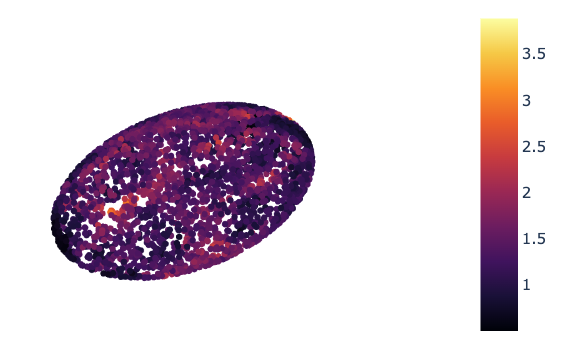
\includegraphics[width=0.3\textwidth]{fig/vol_ellipsoid.png}
        \label{fig:vol_ellip}
    }
    \subfigure[Saddle]{
        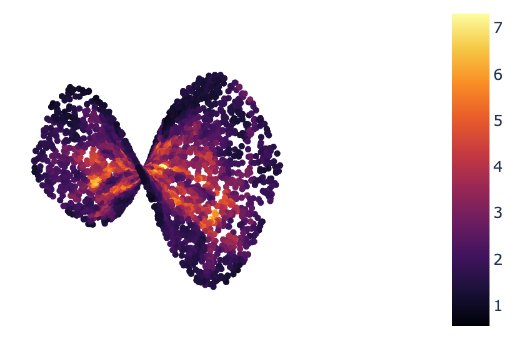
\includegraphics[width=0.3\textwidth]{fig/vol_saddle.png}
        \label{fig:vol_sadd}
    }
    \subfigure[Torus]{
        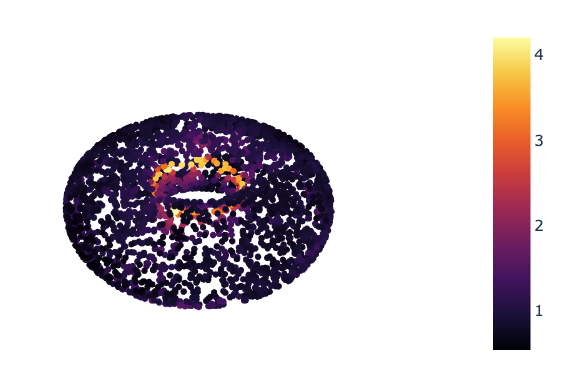
\includegraphics[width=0.3\textwidth]{fig/vol_torus.png}
        \label{fig:vol_tor}
    }
    \caption{Pullback metric enables computation of volume element on the manifold}
    \label{fig:vol}
\end{figure}

\subsection{Generative denoising model}
\par Generating data in the high-dimensional space comes with challenges such as the difficulty to cover the entire population and computational complexity. We make use of the autoencoder we trained: First generate data $\tilde z$ in the latent space, and then use the decoder function to map it to the data space $\tilde x=g(\tilde z)$. For generating data, we use the recently successful denoising diffuion probabilistic model \cite{ho2020denoising,dhariwal2021diffusion}. The model is trained by gradually adding noise $z_{i+1}=z_i+\epsilon_i$ to the data $z_0=z$ for $K$ steps, and learns a denoising function $z'_i=s(z_{i+1})$, and generates by inverting this process from a Gaussian noise $\epsilon_K$. (For details on the loss function please refer to \cite{ho2020denoising,dhariwal2021diffusion}).
\par The advantage of using this latent diffusion model \cite{rombach2022high} with our geometric-aware autoencoder is that we are able to maintain the geometric structures even when generating on the low-dimensional latent space, for example, the generated data has a large coverage on all the branches and clusters (modes) in the latent space, which are mapped to the high-dimensional structures in the data space.

\begin{algorithm}[htbp]
\caption{Generate denoising model with \methodshort}
\begin{algorithmic}[1]
\State \textbf{Start} from Gaussian noise $\epsilon_K \sim \mathcal{N}(0, I_d)$
\State $z_K = \epsilon_K$
\For{$k = K, K-1, \ldots, 0$}
    \State $\epsilon_k \sim \mathcal{N}(0, I_d)$
    \State $z_{k-1} = a_k s(z_k) + b_k \epsilon_k$ \\
    \Comment{$a_k$ and $b_k$ are constants computed with the noise schedule used in training}
\EndFor
\State $x_0 = g(z_0)$
\State \Return $x_0$
\end{algorithmic}
\end{algorithm}

\subsection{Geodesic computation}\label{sec:geodesic}
\par In section \ref{sec:ae} we obtained a pullback metric $g$ from the geometric-aware encoder, by minimizing the curve length under $g$. We use this metric to learn geodesics on the data manifold. Because this metric is defined only on the data manifold which is a subset of the space $\mathbb R^n$, it would be not be able to be applied to the space not on the manifold. Previous methods \cite{fasina2023neural,huguet2022manifold} deal with this by penalizing the curve to be close to existing points in the data, but we argue that this method would be vulnerable to large noise and low-density regions on the manifold. Alternatively, we extend the metric $g$ to the entire space $\mathbb R^n$ with the help of a discriminator that can distinguish points on and off the manifold. We start with generating $N$ high-frequency negative samples $\check x_1,\dots,\check{x_N}$ that are not on the manifold. \xin{explain in appendix}. The discriminator $w$ is a neural network that predicts a score $w(x)$ of how likely the point $x$ is on the data manifold. To get a smooth $w$ such that the prediction score increases as $x$ moves away from the manifold, we use a loss function inspired from Wasserstien GAN \cite{arjovsky2017wasserstein}
\begin{align}
    L_3=\frac{1}{N}\sum_{i=1}^N w(\check x_i)-\frac{1}{N}\sum_{i=1}^N w(x_i)+\operatorname{var}(\{w(x_i),i=1,\dots,N\}),
\end{align}
where the last term stabilizes the predicted score on the positive samples. We in addition apply weight-clipping and spectral normalization to make sure $w$ is smooth and stable. After training, $w$ is rescaled and shifted to the range $[0,1]$. With this discriminator, we propose a function $r$ that maps the data into an dimension-extended latent space $\mathbb R^{d+1}$:
\begin{align}
    r(x)=\left(\begin{matrix}
        e^{c_1(1-w(x))}f(x)\\c_2(1-w(x))
    \end{matrix}\right)\label{expn:extn}
\end{align}
where $c_1,c_2>0$ are hyperparameters.
Figure \ref{fig:extn} shows an illustration of the space. The pullback metric now becomes 
\begin{align}
    g'=r^*d_{\mathbb R^{d+1}}\label{expn:extn_metric}
\end{align} and it is defined on the entire space $\mathbb R^{n}$. Intuitively, (\ref{expn:extn_metric}) guarantees that the cost (length) of moving a point along a curve off the manifold is much smaller than that of moving on the manifold.
\begin{figure}[htbp]
    \centering
    \subfigure[Negative sampling]{
        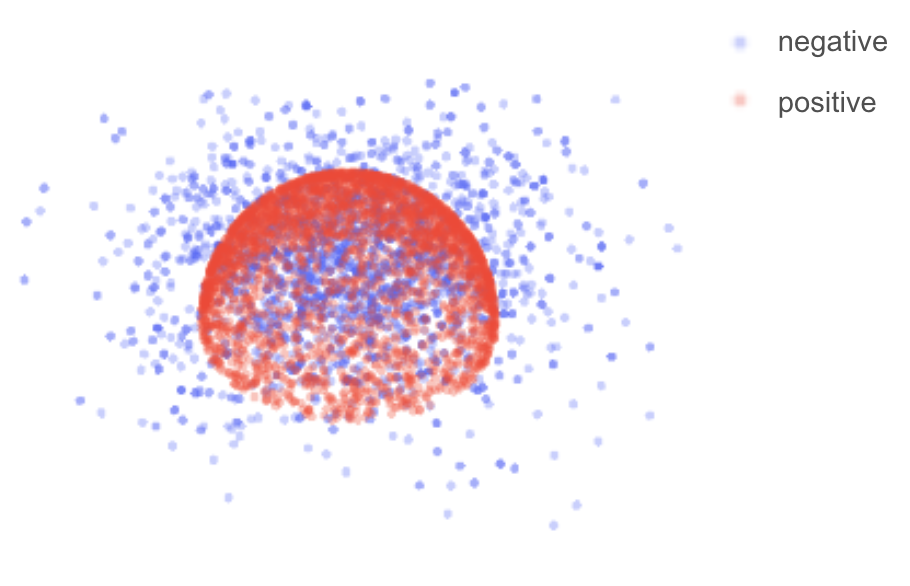
\includegraphics[width=0.3\textwidth]{fig/hemi_negative.png}
        \label{fig:hemi_negative}
    }
    \subfigure[Discriminator]{
        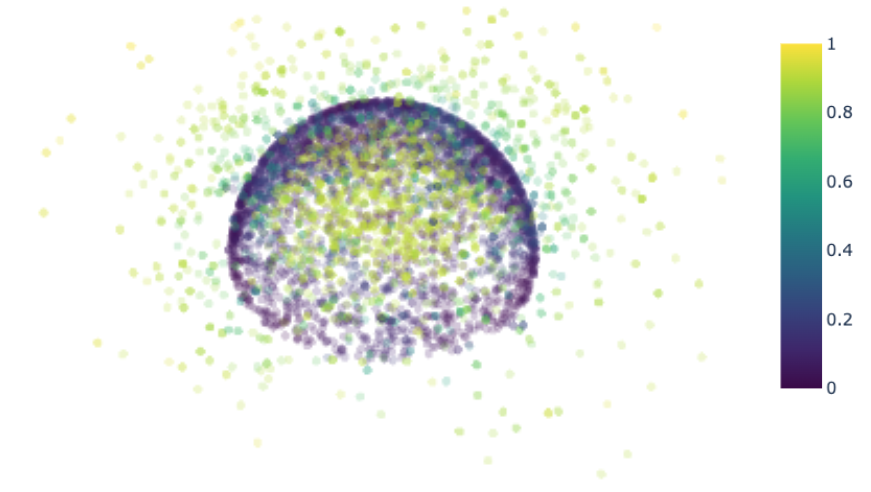
\includegraphics[width=0.3\textwidth]{fig/hemi_disc.png}
        \label{fig:hemi_disc}
    }
    \subfigure[Extended latent space]{
        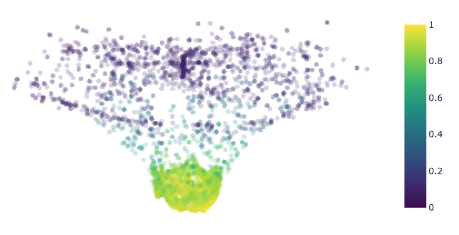
\includegraphics[width=0.3\textwidth]{fig/hemi_extn.png}
        \label{fig:hemi_extn}
    }
    \caption{$r$ maps data space to extended latent space, where the data manifold is mapped to bottom}
    \label{fig:extn}
\end{figure}
\par Next, given two points $x_1,x_2$, we parameterize a curve between them with a neural network. Previous works \cite{fasina2023neural,huguet2022manifold} use neural ODE \cite{chen2018neural} to parameterize the velocity vector of a curve and obtain the curve by numerical integration. However, numerical integration has shown to be slow and thus not scalable to large, high-dimensional datasets, and an additional penalty that the curve reaches the end point needs to be added, making the training more difficult. \xin{add empirical ablation in appendix}. Alternatively, we parameterize the curve $c$ as a non-linear interpolation
\begin{align}
    c(x_0,x_1,t)=tx_1+(1-t)x_0+(1-(2t-1)^2)b(x_0,x_1,t)\label{expn:geob}
\end{align}
where $b$ is a neural network. The boundary condition $c(x_0,x_1,0)=x_0;c(x_0,x_1,1)=x_1$ is satisfied under (\ref{expn:geob}).
\par With this parameterization, we train the curve to minimize the distance under (\ref{expn:extn_metric}). Let $0=t_1<\dots<t_M=1$, we minimize this loss function
\begin{align}
    L_4=\frac{1}{M}\sum_{m=1}^{M}||\nabla r(c(x_0,x_1,t_m))\frac{\partial}{\partial t}c(x_0,x_1,t_m)||_2^2
\end{align}
We summarize the geodesic computation with Algorithm \ref{alg:geod}

\begin{algorithm}[htbp]
\caption{Geodesic computation}
\begin{algorithmic}[1]
\State {\bfseries Input:} encoder $f$, discriminator $w$, $x_0$, $x_1$, $0=t_1<\dots<t_M=1$
\For{$k = K, K-1, \ldots, 0$}
    \State $\epsilon_k \sim \mathcal{N}(0, I_d)$
    \State $z_{k-1} = a_k s(z_k) + b_k \epsilon_k$ \\
    \Comment{$a_k$ and $b_k$ are constants computed with the noise schedule used in training}
\EndFor
\State $x_0 = g(z_0)$
\State \Return $x_0$
\end{algorithmic}\label{alg:geod}
\end{algorithm}
\subsection{Transport populations along geodesics}
\par Inferring optimal transports between populations has gained increasing importance in high-dimensional data analysis, especially in single cell analysis\cite{huguet2022manifold}. In addition, this can be viewed as a paradiagm to generate data along the manifold. We take advantage of \methodshort's geodesic computation, to learn a populational transport such that the points move along geodesics while minimizing total cost.
\par We start by training a 
% \xin{its from fim journal version; dont want to highlight as a key contribution; can write in a as \textit{low-key} as possible way, "we consider a new parameterization, why use this: (ablation study?)"}\\
% \xin{1. some method does that, one is ODE, however its slow/need to force end points there, hence we use this. <at the end> we empirically validated this is faster/no need that loss term.}

\subsection{Generating geodesics between populations}
We can also transport point cloud data along geodesics at the population level\cite{fasina2023neural}.
\par We do this iteratively: in each iteration, we compute the optimal transport pairing of the points, and retrain the geodesics between the pairs, until the total length of the curves are minimized. For more details, see Algorithm \ref{alg:mbotcfm}.

\begin{algorithm}[htbp]
  \caption{Minibatch Geodesic FM}
  \label{alg:mbotcfm}
\begin{algorithmic}
\State {\bfseries Input:} Empirical or samplable distributions $q_0,q_1$, variance schedule $\sigma_k(t)$, batch size $b$, initial curve network $C_\theta$, metric $g$, $T$ times to sample.
\While{Training}
\Comment{Sample batches of size $b$ \textit{i.i.d.} from the datasets}
\State $\vx_0 \sim q_0(\vx_0); \quad \vx_1 \sim q_1(\vx_1)$
\State $\pi \gets \mathrm{OT}(\vx_1, \vx_0)$
\State $(\vx_0, \vx_1) \sim \pi$
\State $\vt \sim (\mathcal{U}(0, 1))^T$
\State $L(C_\theta) \gets C_\theta(\vx_0, \vx_1, \vt)$ \Comment{Length of current curve}
\State $\theta \gets \mathrm{Update}(\theta, \nabla_\theta L(\gamma))$
\EndWhile
\State \Return $C_\theta$
\end{algorithmic}
\end{algorithm}

\section{Results}
\subsection{Geometric-Aware Autoencoder}
In this section, we first provide a quantitative evaluation of \methodshort's embedding and reconstruction. Then, we visualize the embeddings for a qualitative assessment. Lastly, we show that \methodshort's pull-back metric provides curvature, a geometric quantity on the manifold. We compare \methodshort with autoencoder and with exponential distance decay weight. 
\subsubsection{Quantitative evaluation on embedding}
\par We generated single cell RNA-sequence datasets with different data generation and noise settings using splatter\cite{zappia2017splatter}, so that we can compare the output of \methodshort with the ground truth.
\par We first compare the distance from our embedding with PHATE, the distance we trained the model with. The accuracy is defined as
\begin{align}
    \text{Distance Accuracy}=\frac{2}{N(N-1)}\sum_{i<j}\Bigg|\frac{||z_i-z_j||^2_2-d_{ij}^2}{d^2_{ij}}\Bigg|
\end{align}
Where $z_i=f(x_i)$ is the output of the encoder, and $d_{ij}$ is the PHATE distance between $x_i$ and $x_j$.

\begin{figure}[htbp]
    \centering
    
\includegraphics[width=0.5\textwidth]{fig/PLACEHOLDER.png}
    \caption{\methodshort matches distances with high accuracy}
    \label{fig:dist_acc}
\end{figure}
\par In Figure \ref{fig:dist_acc}, we show that \methodshort has high accruacy for distance preservation at different settings.
\par DEMaP\cite{moon2019visualizing} measures how well the embedding preserves geodesic distances. It first computes the graph shortest path distance $d_{ij}^{\text{Dijkstra}}$ between each pair of points on the noiseless data as ground truth using Dijkstra's algorithm, and then computes the correlation between pairwise distances in the embedding space and the ground truth.
\begin{align}
    \text{DEMaP}=\frac{2}{N(N-1)}\sum_{i<j}\operatorname{Corr}(||z_i-z_j||^2_2-(d_{ij}^{\text{Dijkstra}})^2)
\end{align}
where $\operatorname{Corr}$ denotes Pearson correlation.
In Figure \ref{fig:demap}, we show that \methodshort has good preservation of geodesic distances, with high DEMaP score at various settings. Moreover, the score is close to that of PHATE, which is the distance the model is trained with.
\begin{figure}[htbp]
    \centering
    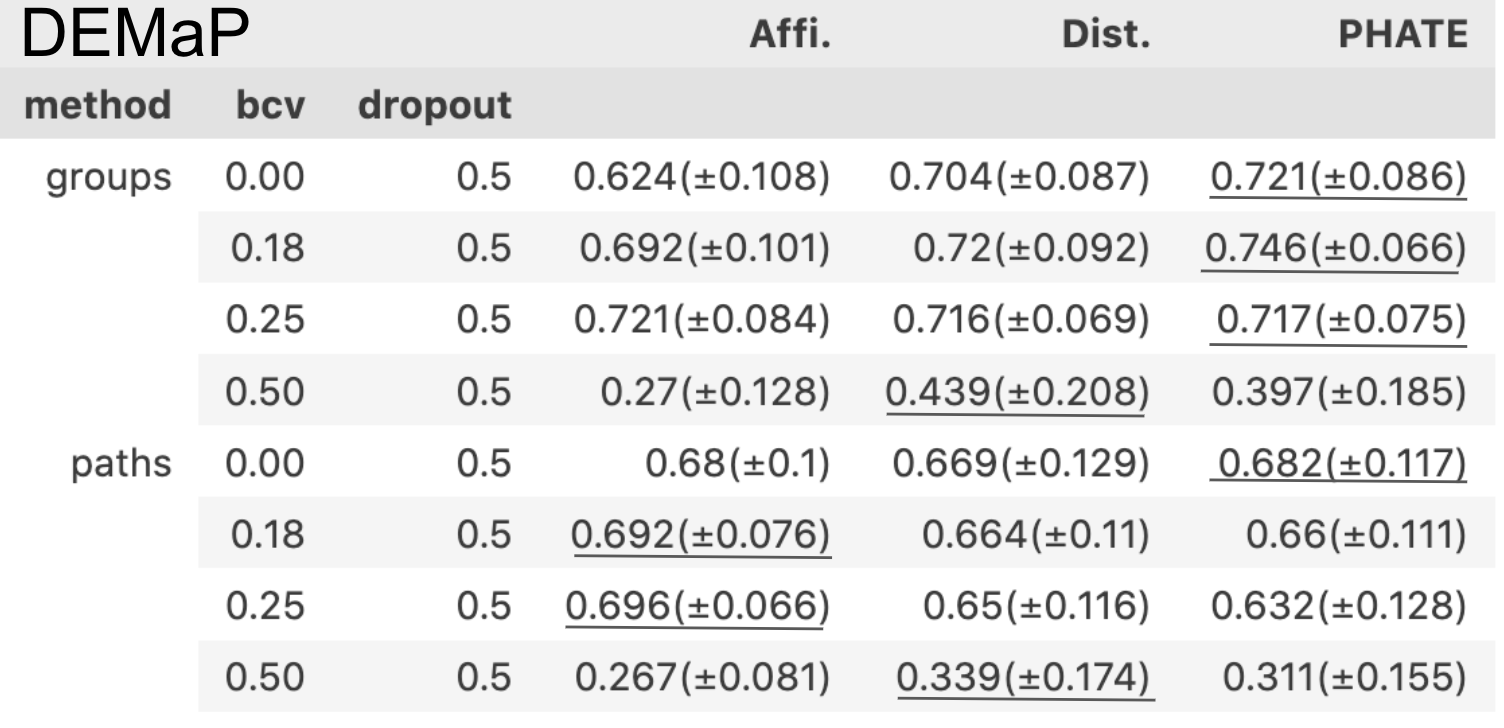
\includegraphics[width=0.5\textwidth]{fig/demap.png}
    \caption{DEMaP shows \methodshort recovers geodesic distances provided by PHATE}
    \label{fig:demap}
\end{figure}
\par To evaluate the reconstruction of \methodshort, we compute the mean squared error, and two novel criteria called \textit{DGCS (Denoised Gene Correlation Score)} and \textit{DRS (Denoised Reconstruction Score)}. Due to the noisy nature of the single cell data, we would not want a perfect reconstruction of the data, but would like to recover the gene trends in the denoised data. We first apply MAGIC\cite{van2018recovering} to denoise the data, and compare the pearson correlation between each gene pair in the denoised data and in the reconstructed data. (\methodshort is trained on the PCA space so we use inverse PCA to map the reconstructed points back to the gene space.) In addition, we also compute the mean pearson correlation between each gene in the denoised data and that gene in the reconstructed data.
\begin{align}
    \text{DGCS}=&\frac{2}{N_{\text{gene}}(N_{\text{gene}}-1)}\sum_{i<j}(\operatorname{Corr}(y_i,y_j)-\operatorname{Corr}(y^{\text{MAGIC}}_i,y^{\text{MAGIC}}_j))^2\\
    \text{DRS}=&\frac{1}{N_{\text{gene}}}\sum_{i=1}^{N_{\text{gene}}}\operatorname{Corr}(y_i,y^{\text{MAGIC}}_i)
\end{align}
where $y_i=\operatorname{PCA^{-1}}(g(f(x_i))$, $y^{\text{MAGIC}}_i=\operatorname{PCA^{-1}}(\operatorname{MAGIC}(x_i))$
\par Figure \ref{fig:recon_score} shows \methodshort captures gene-gene correlation and has high correlation with denoised data.
\begin{figure}[htbp]
    \centering
    
\includegraphics[width=0.5\textwidth]{fig/PLACEHOLDER.png}
    \caption{Reconstruction metrics show \methodshort captures gene-gene correlation and has high correlation with denoised data}
    \label{fig:recon_score}
\end{figure}
\subsubsection{Visualizations}
\par In Figure \ref{fig:embedding} we visualize \methodshort's 2D embeddings trained on real-world scRNAseq data (Embryo-body\cite{moon2019visualizing} and SEA-AD\cite{gabitto2023integrated}). We compared the PHATE embedding, and \methodshort trained without and with the exponential distance decay. We can see that the exponential distance decay helps the model better capture the local distances, and thus better preserves the manifold structure.
\par With the pullback metric from \methodshort's encoder, we compute the volume by taking the pseudo-determinant of the metric matrix at each point, and visualize it on toy datasets (Figure \ref{fig:volume})
\begin{figure}[htbp]
    \centering
    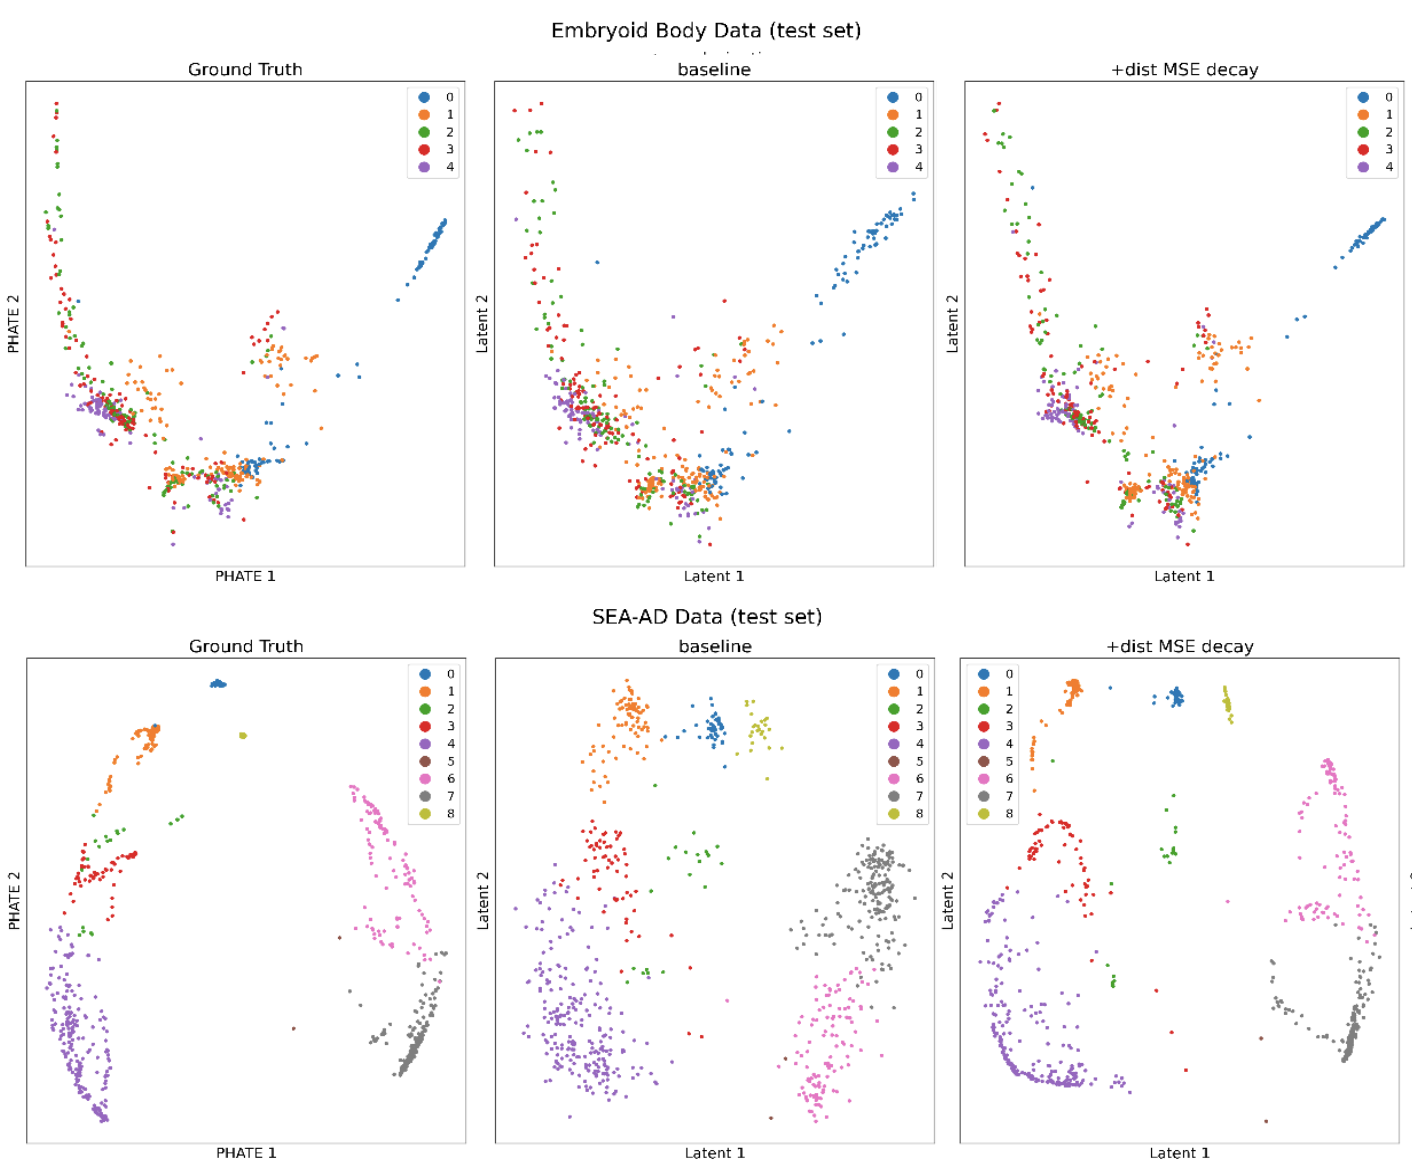
\includegraphics[width=0.5\textwidth]{fig/visualization.png}
    \caption{Visualization of the embedding}
    \label{fig:embedding}
\end{figure}
\begin{figure}[htbp]
    \centering
    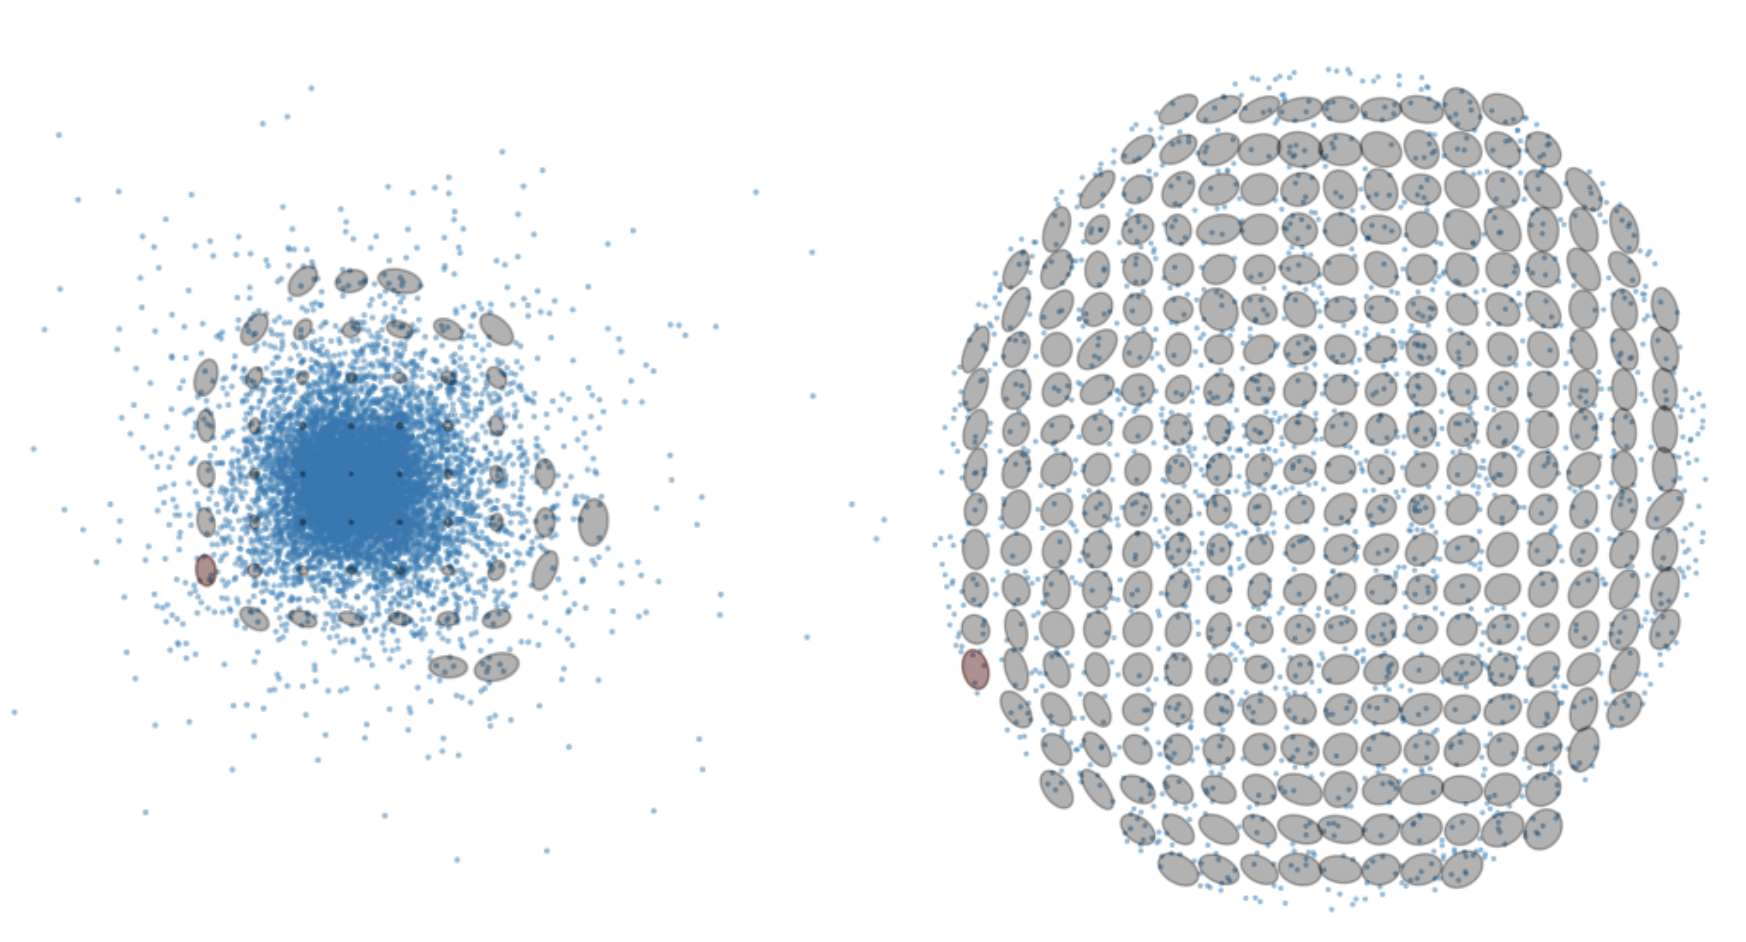
\includegraphics[width=0.5\textwidth]{fig/volume.png}
    \caption{Volume computed with the pullback metric on sphere, torus, and saddle}
    \label{fig:volume}
\end{figure}
\begin{figure}[htbp]
    \centering
    
\includegraphics[width=0.5\textwidth]{fig/PLACEHOLDER.png}
    \caption{Curvature computed with the pullback metric}
    \label{fig:volume}
\end{figure}
\subsection{Generative Denoising Model}
\par We evaluate the generated points of the Generative Denoising Model on the latent space and the reconstruction space. On the latent space, we compute the 2-Wasserstein distance between the generated data and the test data to show \methodshort can generate a population of data with a distribution close to the true data, and does not exactly reproduce the training data. On the reconstrunction space, we compute DGCS to show the generated data has the same gene-gene correlation trend as the true data. In Figure \ref{fig:dm_eval} We 
\par In Figure \ref{fig:dm_eval} we plotted the metrics on generated points as we increase of latent space dimensions. In Figure \ref{fig:gen_corr} We plot the gene-gene correlations of the top 100 highly variable genes for a qualitative evaluation.
\begin{figure}[htbp]
    \centering
    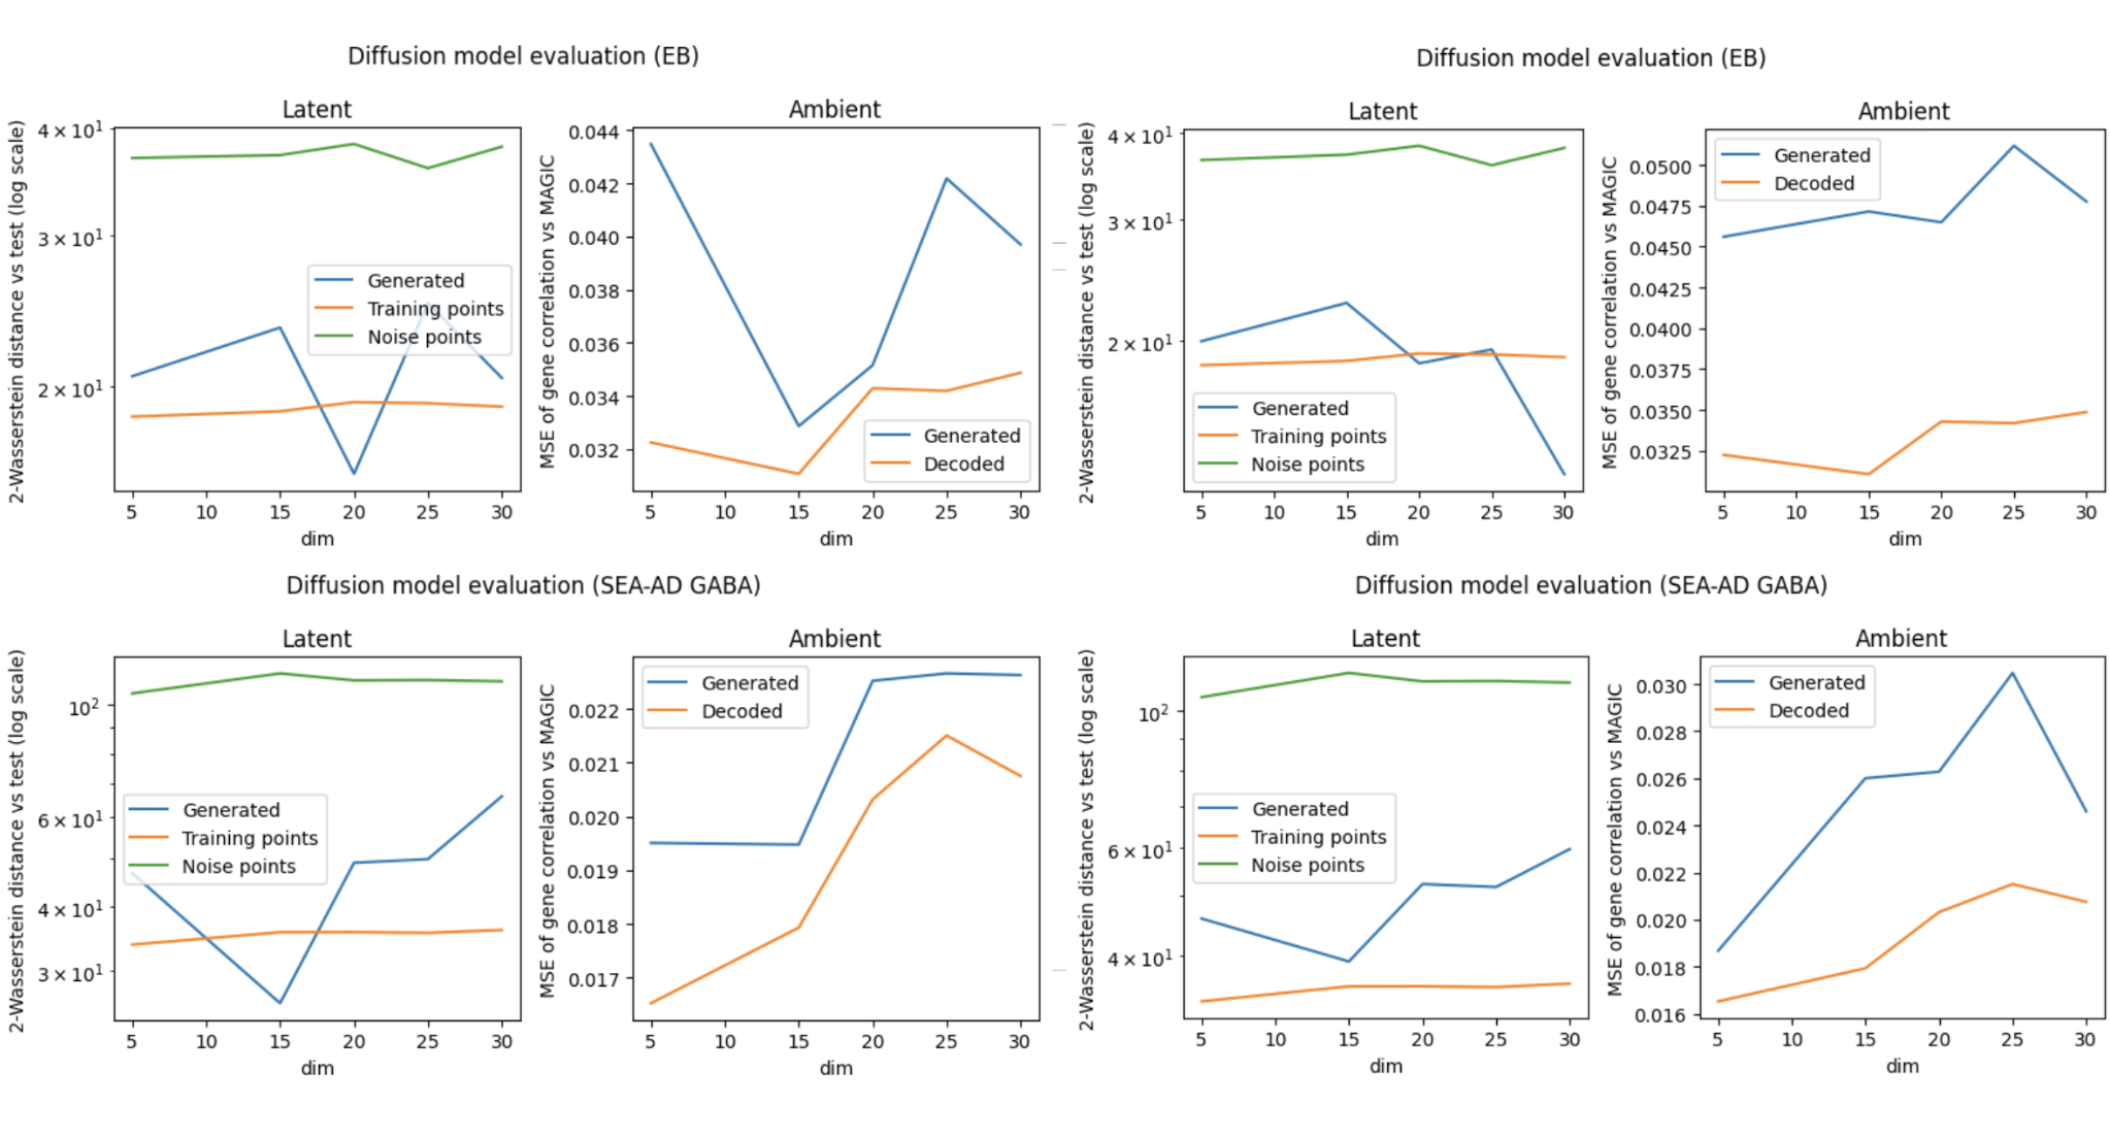
\includegraphics[width=0.5\textwidth]{fig/dm_eval.png}
    \caption{Evaluation metrics on generated points as dimensions of latent space increase.}
    \label{fig:dm_eval}
\end{figure}
\begin{figure}[htbp]
    \centering
    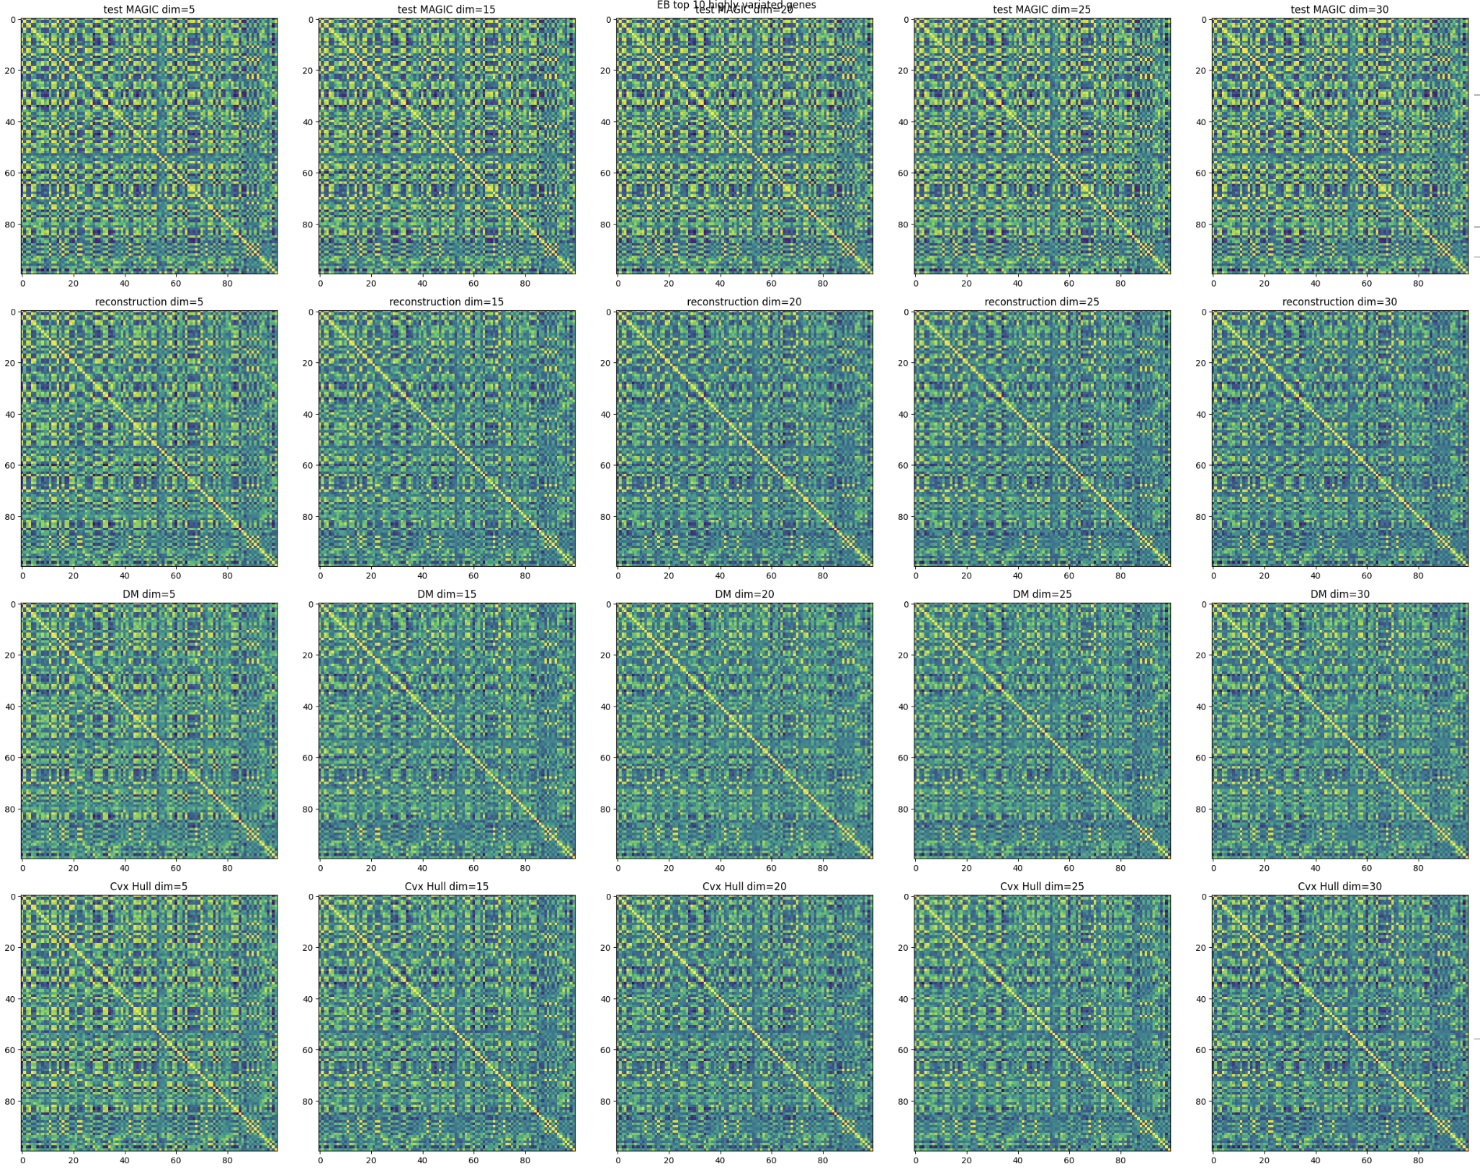
\includegraphics[width=0.5\textwidth]{fig/gen_corr.png}
    \caption{Gene-gene correlation of generated points compared with that of MAGIC}
    \label{fig:gen_corr}
\end{figure}

\subsection{Pointwise Geodesic computation}
\par We first visualize our discriminator and extended-dimension embedding on the toy dataset. (Figures \ref{fig:discriminator},\ref{fig:offmfdr})
\begin{figure}[htbp]
    \centering
    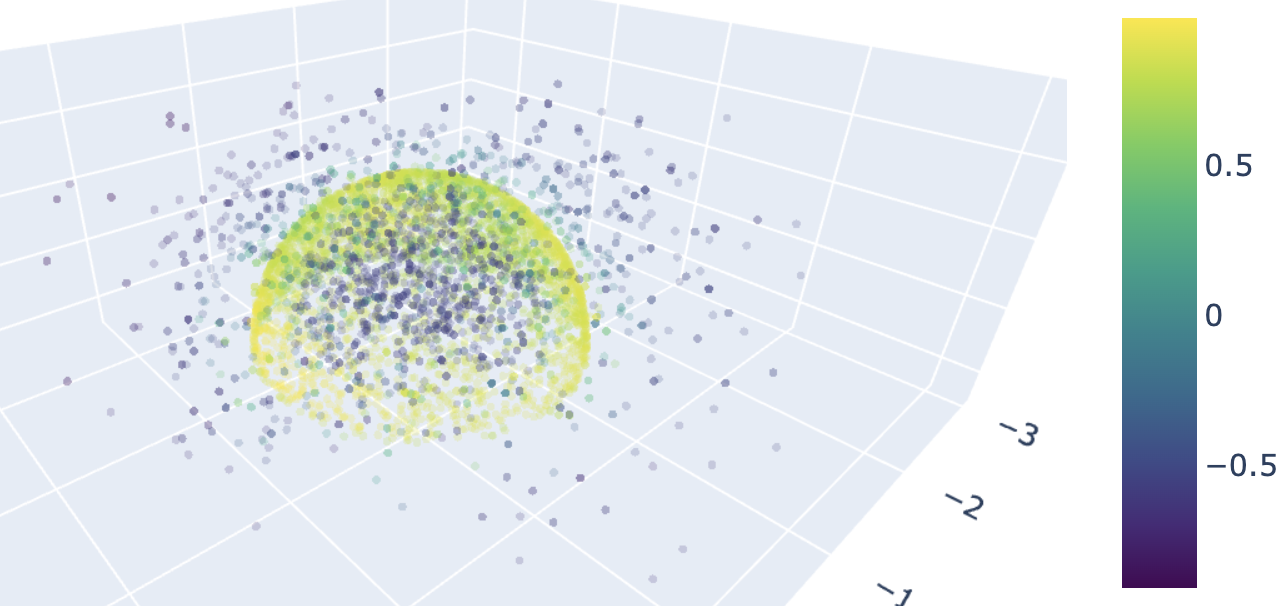
\includegraphics[width=0.5\textwidth]{fig/discriminator.png}
    \caption{Discriminator prediction on toy data with negative sampling}
    \label{fig:discriminator}
\end{figure}

\begin{figure}[htbp]
    \centering
    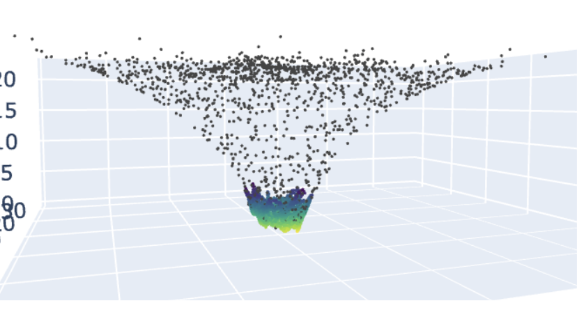
\includegraphics[width=0.5\textwidth]{fig/offmfdr.png}
    \caption{Extended space for off-manifold data}
    \label{fig:offmfdr}
\end{figure}

\par Then we visualize the geodesic learned on toy datasets in Figure \ref{fig:geod_toy}. The geodesics learned by \methodshort is straight when examined by the eye. In Figure \ref{fig:geod_eb}, we show the geodesic learned on the Embryo Body data. The starting point correspond to time point 0 of the EB, while the ending points are selected in each time bin where the sample is collected. The geodesic learned agrees with the biological understanding of the data, which shows the capability of \methodshort to apply to real-world data.
\par In Figure \ref{fig:geod_metrics}, we compute two metrics for the geodesic: We first obtain the ground truth geodesics and their lengths using the analytical expressions of the manifolds, if available, or using the Dijkstra's algorithm. We then compute the geodesic with \methodshort, and compute their lengths. We compute the correlation of the geodesic length with the ground truth, as well as the average minimal distance of the points on \methodshort's geodesic to the true geodesic. The result shows \methodshort learns a curve that is close to the true geodesic, with a length closest to the shortest length.

\begin{figure}[htbp]
    \centering
    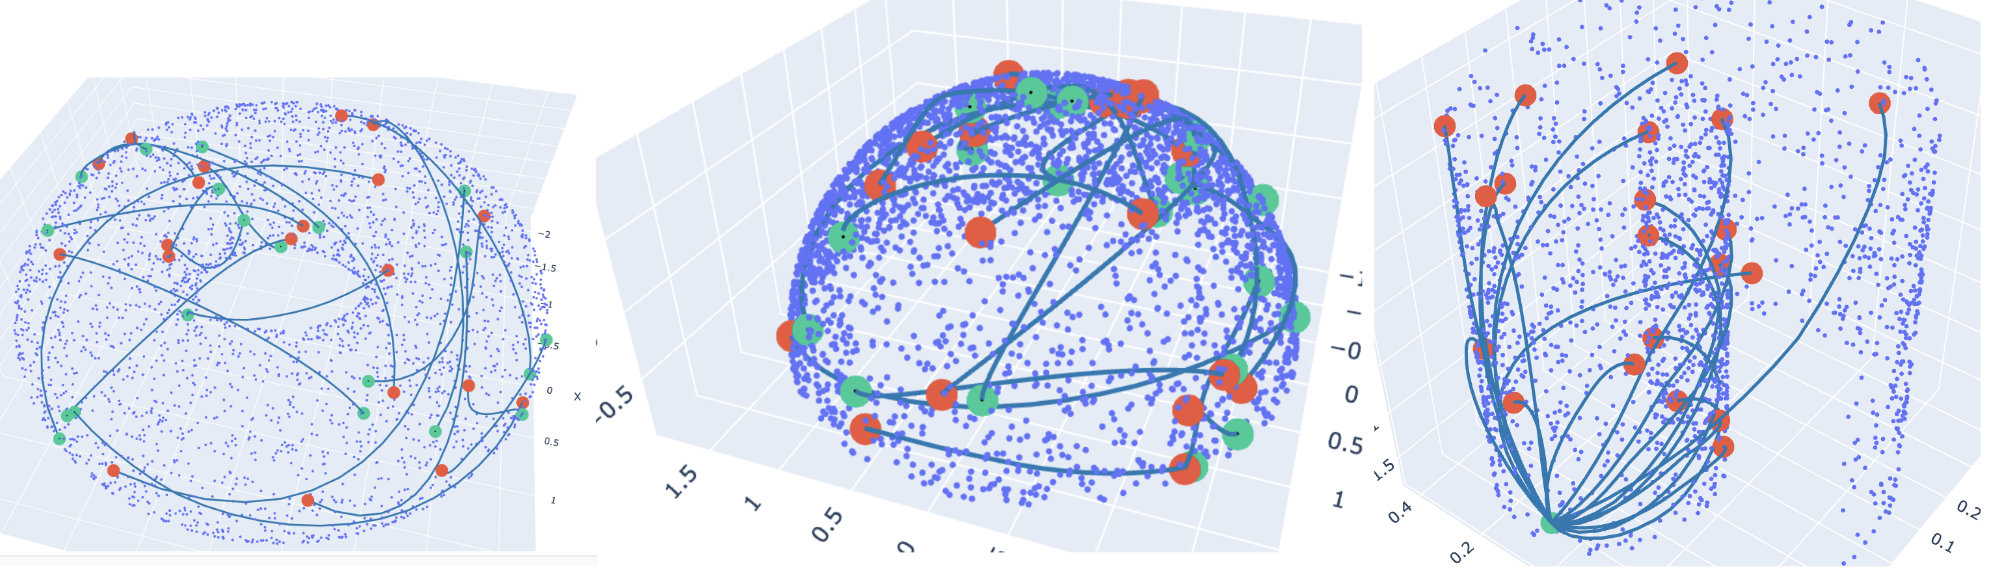
\includegraphics[width=0.5\textwidth]{fig/geod_toy.png}
    \caption{Geodesic on toy manifolds}
    \label{fig:geod_toy}
\end{figure}

\begin{figure}[htbp]
    \centering
    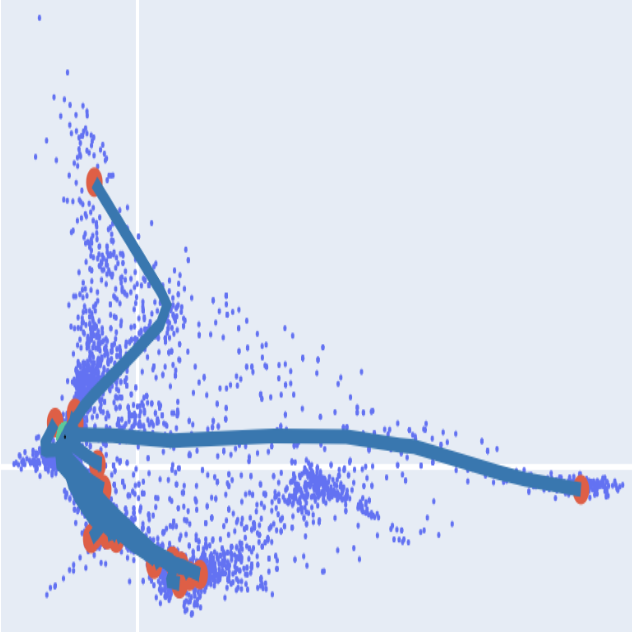
\includegraphics[width=0.5\textwidth]{fig/geod_eb.png}
    \caption{Geodesic on Embryo Body dataset}
    \label{fig:geod_eb}
\end{figure}

\begin{figure}[htbp]
    \centering
    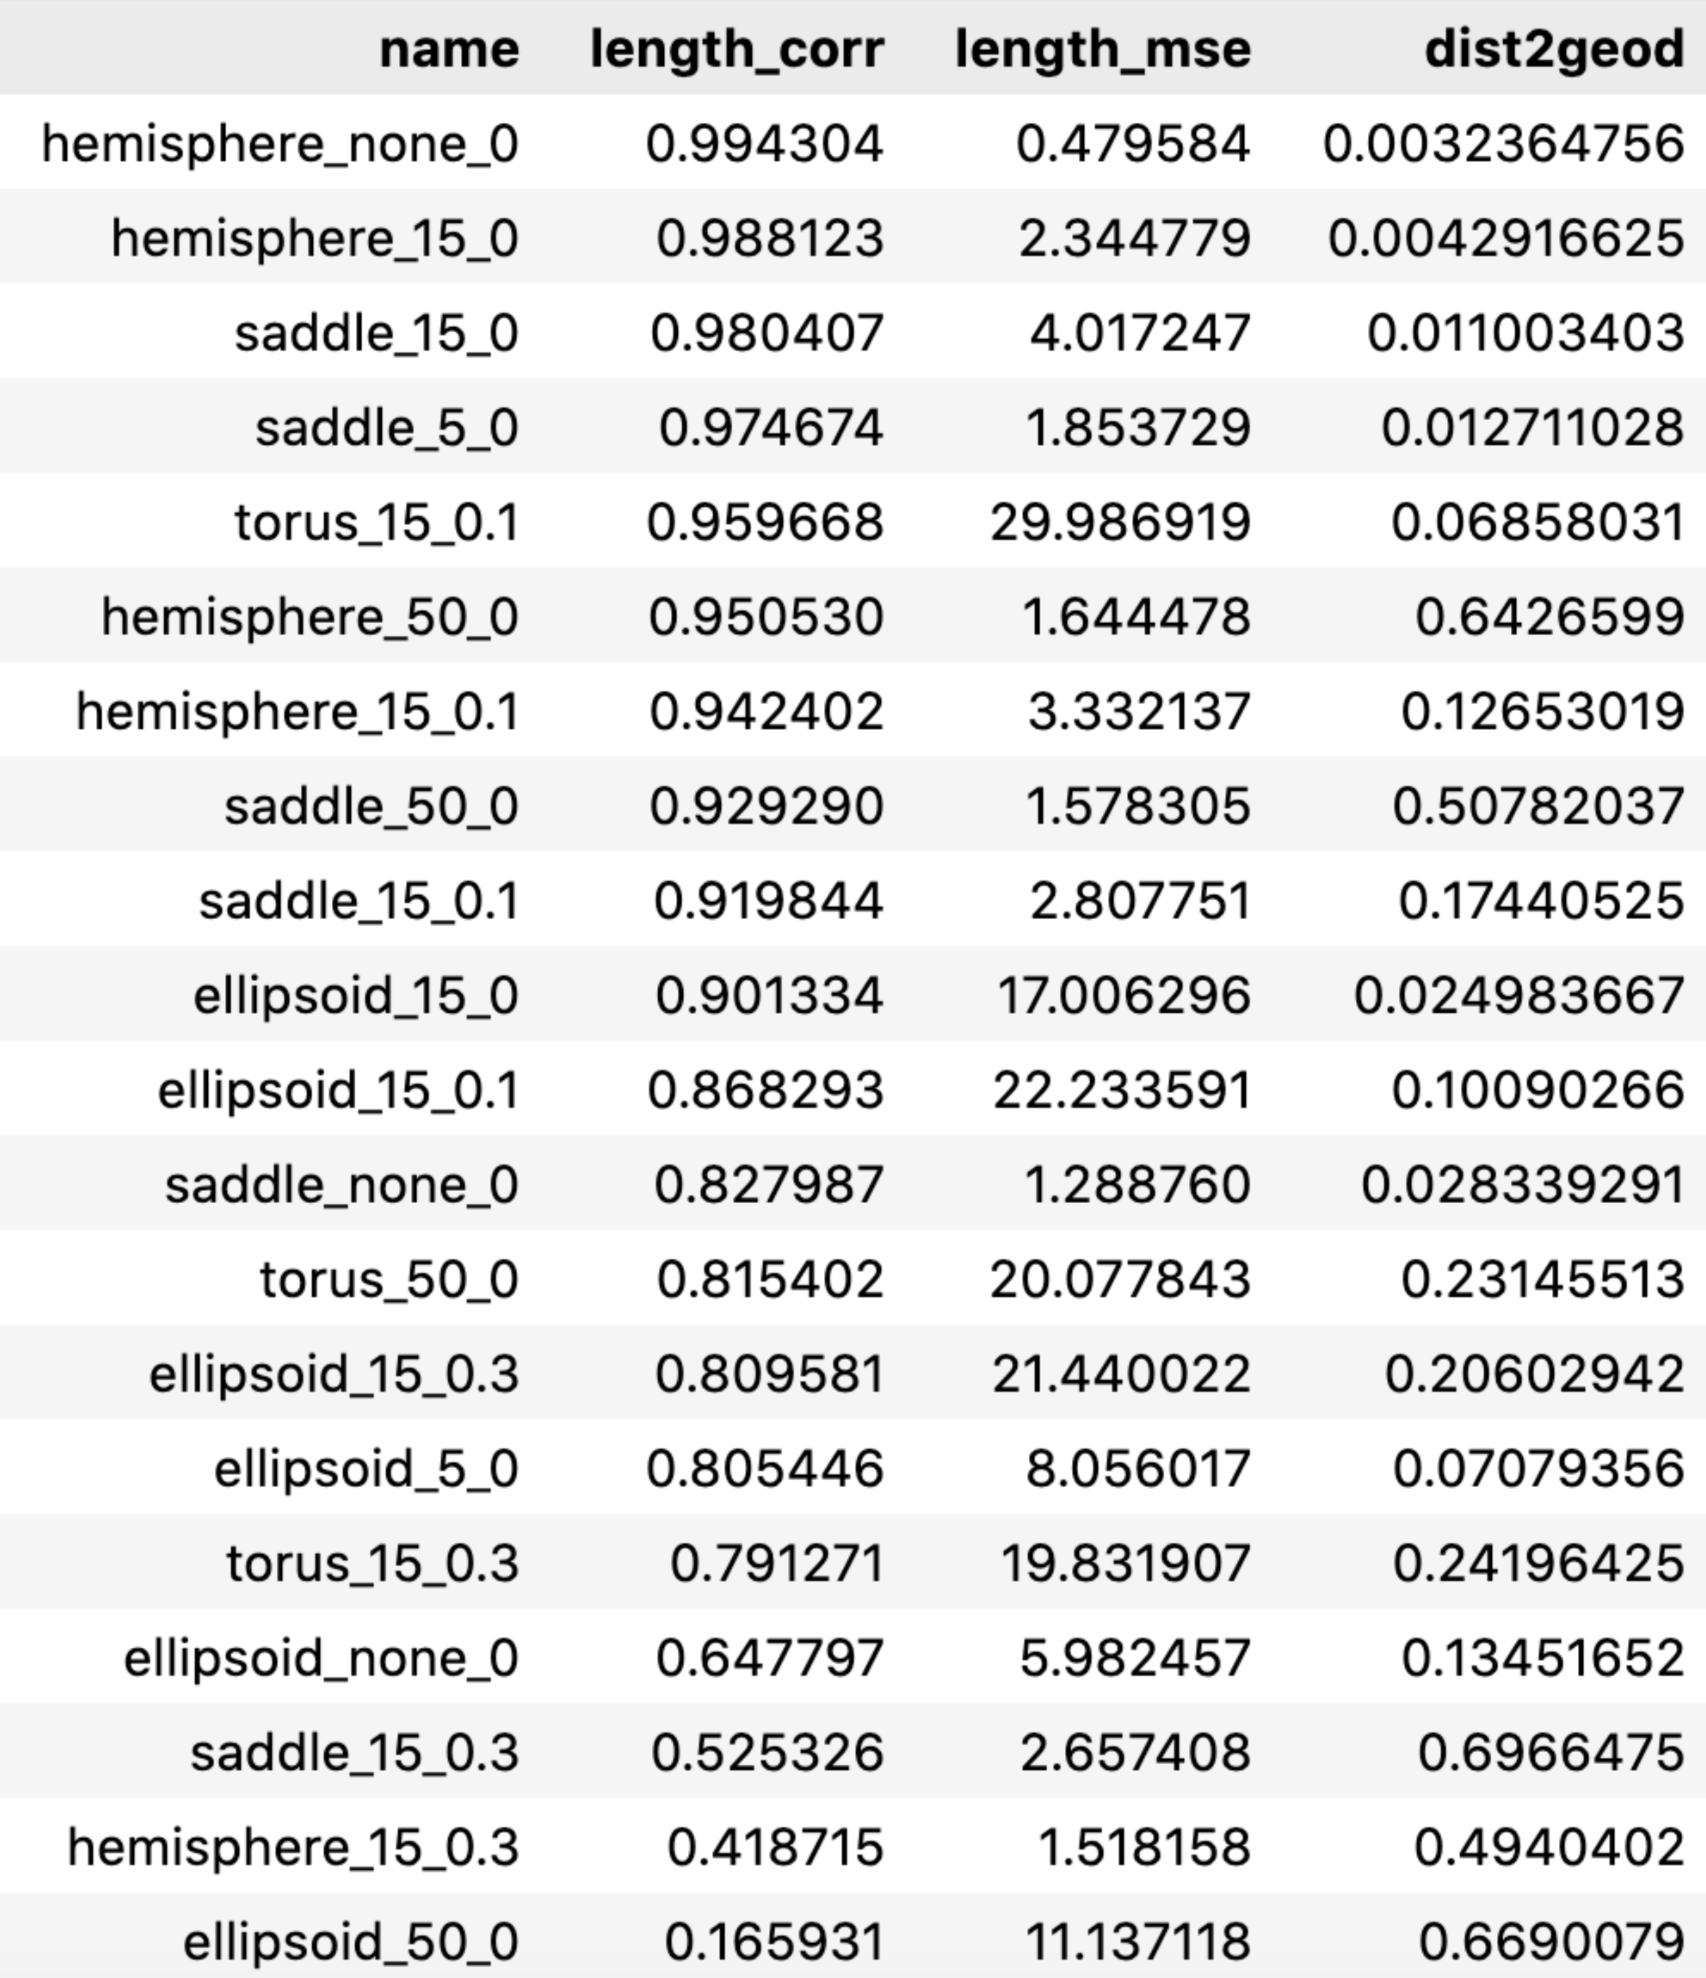
\includegraphics[width=0.5\textwidth]{fig/geod_metrics.png}
    \caption{Evaluation metrics on geodesics}
    \label{fig:geod_metrics}
\end{figure}
\subsection{Population-wise Geodesic Generation}
\par We learned the population-wise geodesics with the optimal pairing on a toy sphere dataset. Figure \ref{fig:latent_only_2} shows the learned geodesics on the latent space, and compared with flow-matching without the metric, the geodesics \methodshort learns are closer to the true geodesic.
\begin{figure}[htbp]
    \centering
    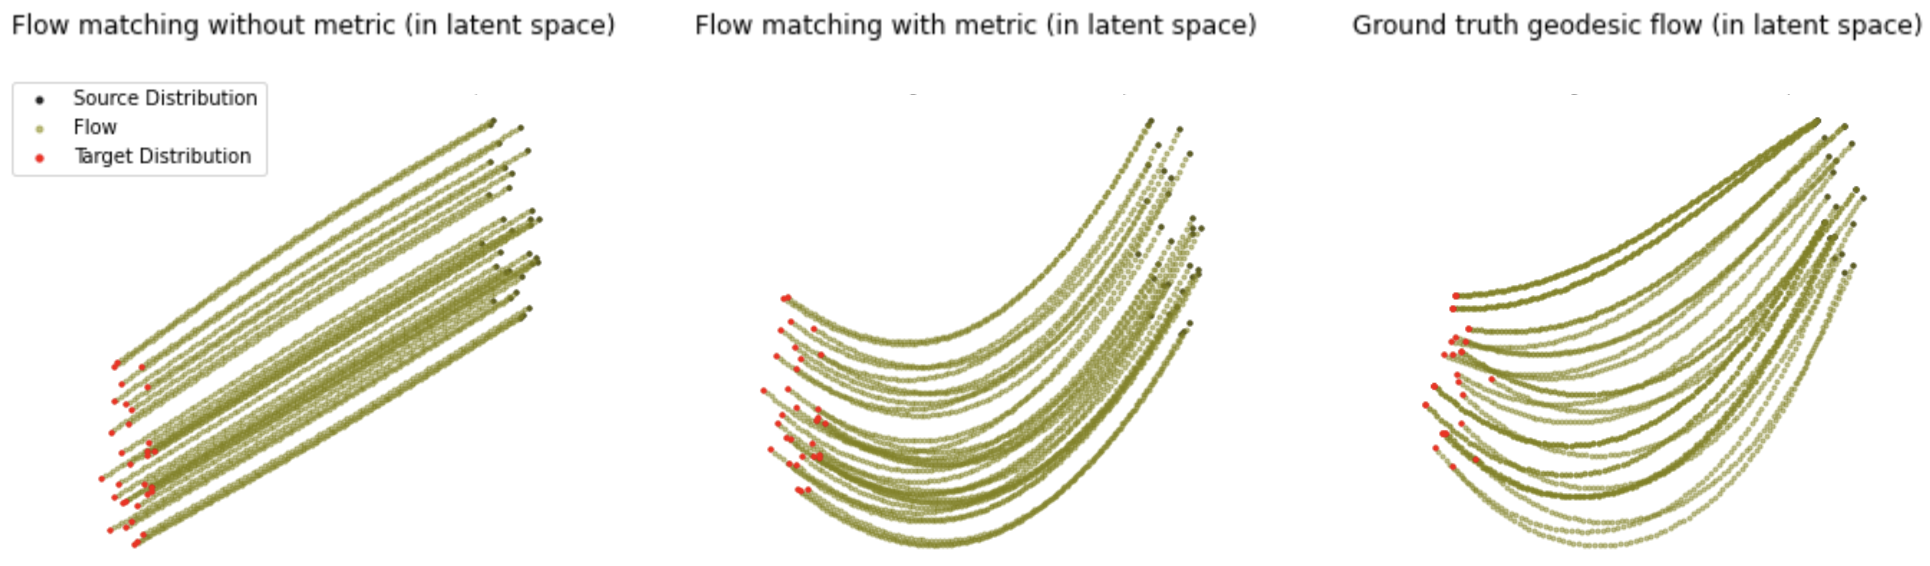
\includegraphics[width=0.5\textwidth]{fig/latent_only_2.png}
    \caption{Population-wise geodesic generated on toy manifold}
    \label{fig:latent_only_2}
\end{figure}

\section{Related Work}
\par Several prior works have been done on learning continuous metrics in data ambient space. Neural FIM \cite{fasina2023neural} learns the Fisher Information Metric from point cloud data by matching Jensen-Shannon divergence between rows of distribution in a latent statistical manifold with Jensen-Shannon divergence between rows of diffusion probability from PHATE operator. 


\section{Conclusion}
\par In this paper, we propose a geometric-aware generative autoencoder (GAGA) that preserves geometry in latent embeddings and can generate news points on the data manifold, along the geodesics, and at the population levels. We circumvent the limitations of existing manifold learning methods by training generalizable geometric-aware neural network embeddings, and learning non-euclidean metric on data space via Riemannian pullback metric.
%\newpage

%\clearpage
\bibliographystyle{plainnat}
%\bibliography{ref}
\bibliography{ref}



\end{document}